\documentclass[a4paper, 9pt]{beamer}

\usepackage{preambolo}


\begin{document}
	\begin{frame}
		\titlepage
	\end{frame}
	
	\begin{frame}{{Accelerazione}}
		\centering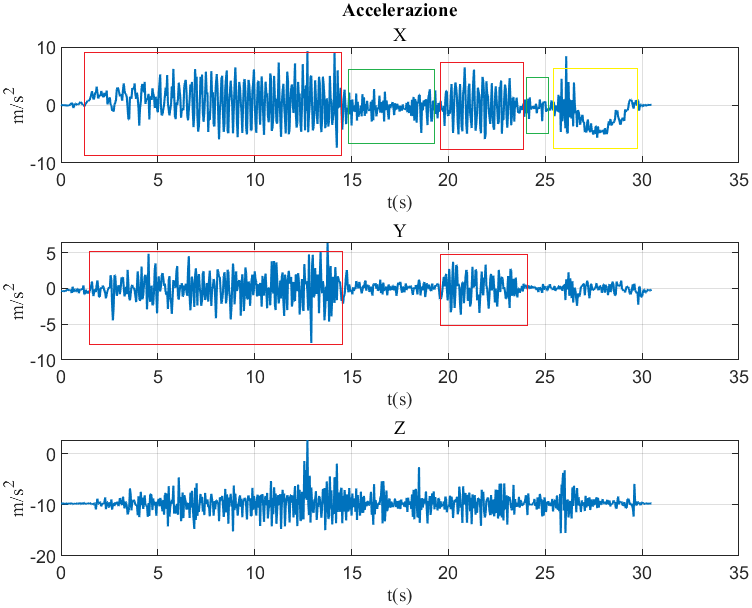
\includegraphics[height=.6\textheight]{figure/esempio_accXY}
		
		\vspace{.05\textheight}
		Dati raccolti dall'accelerometro durante una \textcolor{blue}{\textbf{pedalata forte}}.
		
		Nel riquadro \textcolor{red}{\textbf{rosso}} si può vedere quando la bicicletta \textcolor{red}{\textbf{accelera}}.
		
		Nel riquadro \textcolor{green}{\textbf{verde}} il ciclista \textcolor{green}{\textbf{non pedala}}.
		
		Nel riquadro \textcolor{yellow}{\textbf{giallo}} il ciclista \textcolor{yellow}{\textbf{frena}}.
	\end{frame}
	
	\begin{frame}{{Piano/Forte}}
		\centering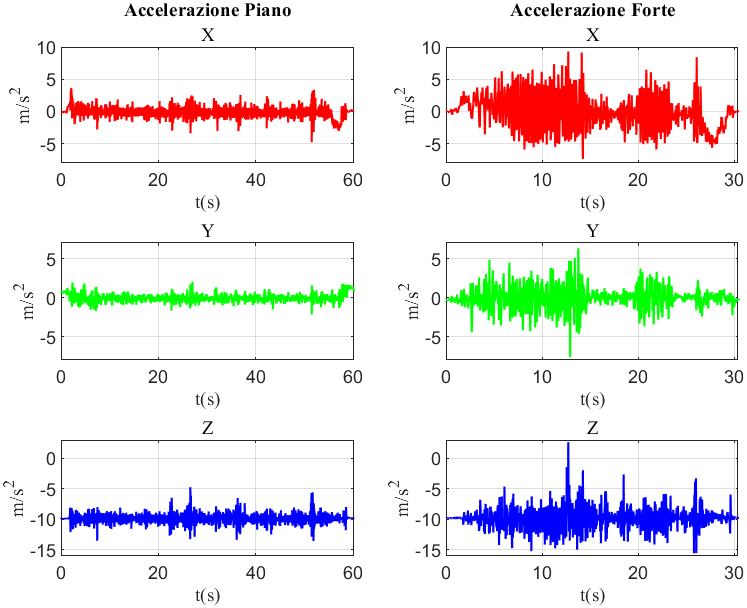
\includegraphics[height=.5\textheight]{figure/lungaFP_accXY}
		
		\vspace{.05\textheight}
		Misure di accelerazione di una \textbf{pedalata piano} (sinistra) e una \textbf{pedalata forte} (destra).
		
		Al fine di stabilire se il ciclista sta pedalando forte o piano è sufficiente considerare gli assi \textcolor{red}{\textbf{X}} e \textcolor{green}{\textbf{Y}}.
		\newline
		\newline
		\textbf{Gli indicatori seguenti sono stati ottenuti dai dati appena presentati}.
	\end{frame}
	
	\begin{frame}{{Accelerazione e Media Accelerazione X}}
			\centering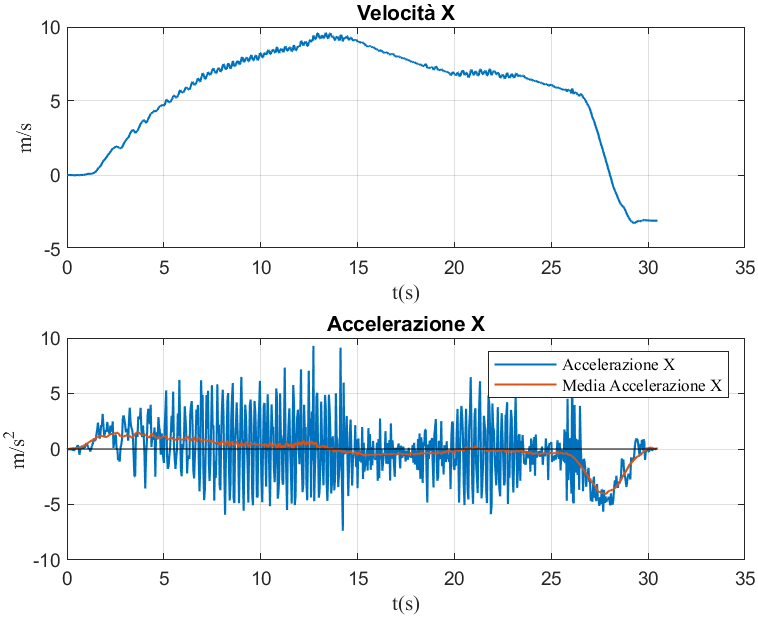
\includegraphics[height=.65\textheight]{figure/MediaAccX}
			\vspace{.05\textheight}
			
			Da questa immagine si può notare come all'aumentare della velocità sia sempre più difficile far accelerare la bicicletta.		
	\end{frame}
	
	\begin{frame}{{Accelerazione Media}}
		\centering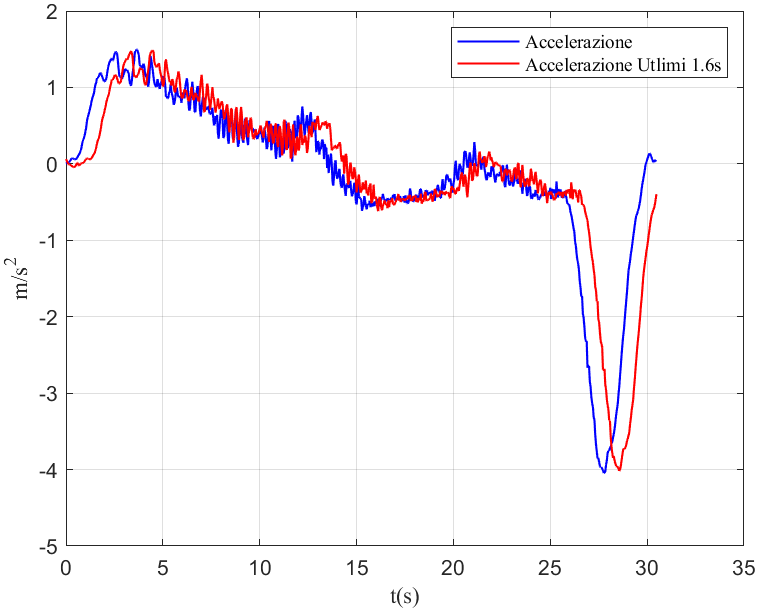
\includegraphics[height=.55\textheight]{figure/mediaVSmediaPost}
		
		\vspace{.05\textheight}
		In \textcolor{blue}{\textbf{blu}} l'accelerazione media dei \textcolor{blue}{\textbf{20 dati precedenti}} (0.8s) e dei \textcolor{blue}{\textbf{20 dati successivi}} ad ogni valore di x.
		
		In \textcolor{red}{\textbf{rosso}} l'accelerazione media dei \textcolor{red}{\textbf{40 dati precedenti}} (1.6s).
		
		I \textbf{prossimi indicatori} saranno tutti presi tenendo in considerazione gli \textbf{ultimi 40 dati}.
		
	\end{frame}
	
	\begin{frame}{{Media Accelerazione X}}
		\centering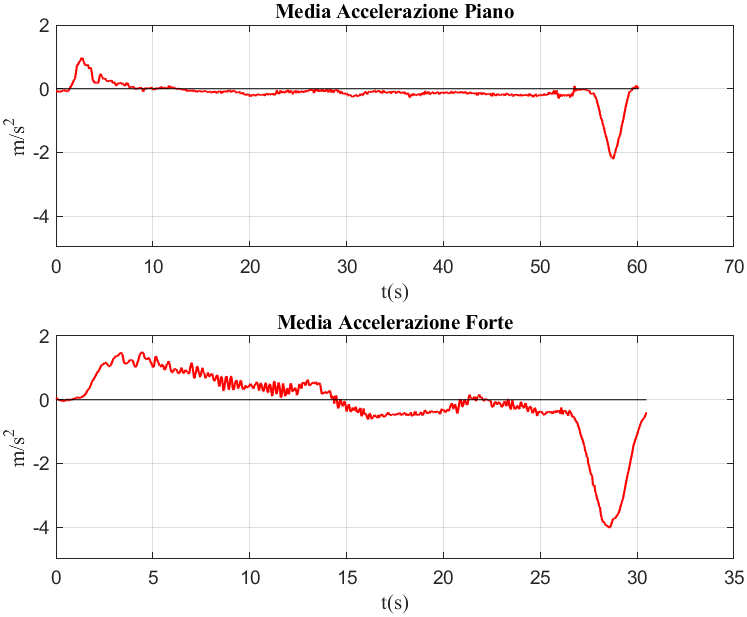
\includegraphics[height=.6\textheight]{figure/lungaFP_mediaAccX}
		\vspace{.05\textheight}
	
		Accelerazione X media degli ultimi 1.6s. Dal grafico si può notare come in caso di pedalata forte i valori di accelerazione si mantengono più alti per un periodo di tempo più lungo.
		
		Oltre a evidenziare l'\textbf{accelerazione} questo indicatore evidenzia anche le \textbf{frenate}.
	\end{frame}
	
	\begin{frame}{{Media Accelerazione Y}}
		\centering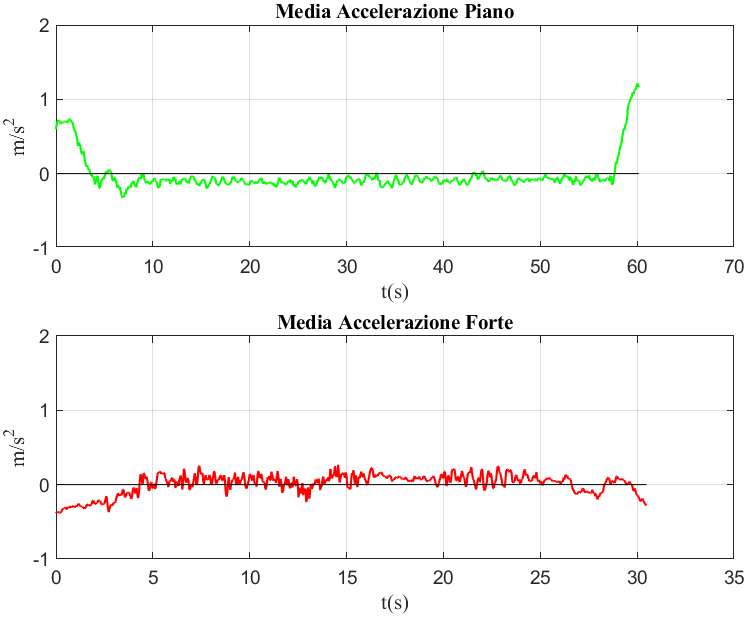
\includegraphics[height=.6\textheight]{figure/lungaFP_mediaAccY}
		\vspace{.05\textheight}
		
		Accelerazione Y media degli ultimi 1.6s. Dal grafico si può notare come questo indicatore non sia particolarmente utile per stabilire se il ciclista sta pedalando piano o forte.
	\end{frame}
	
	\begin{frame}{{Valor Medio Rettificato X}}
		\centering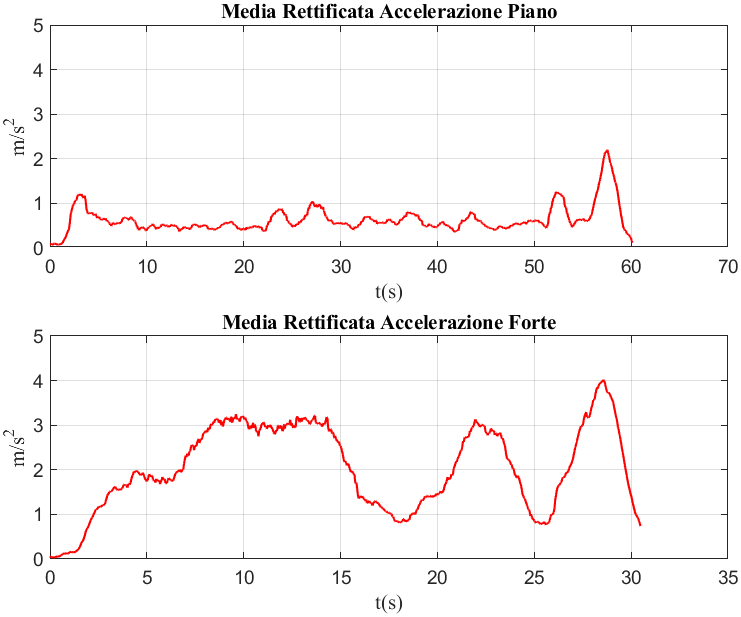
\includegraphics[height=.65\textheight]{figure/lungaFP_arvAccX}
		
		\vspace{.05\textheight}
		Come visibile in figura, questo indicatore evidenzia in \textbf{egual misura} sia le \textbf{accelerazioni} che le \textbf{frenate}.
	\end{frame}
	
	\begin{frame}{{Valor Medio Rettificato Y}}
		\centering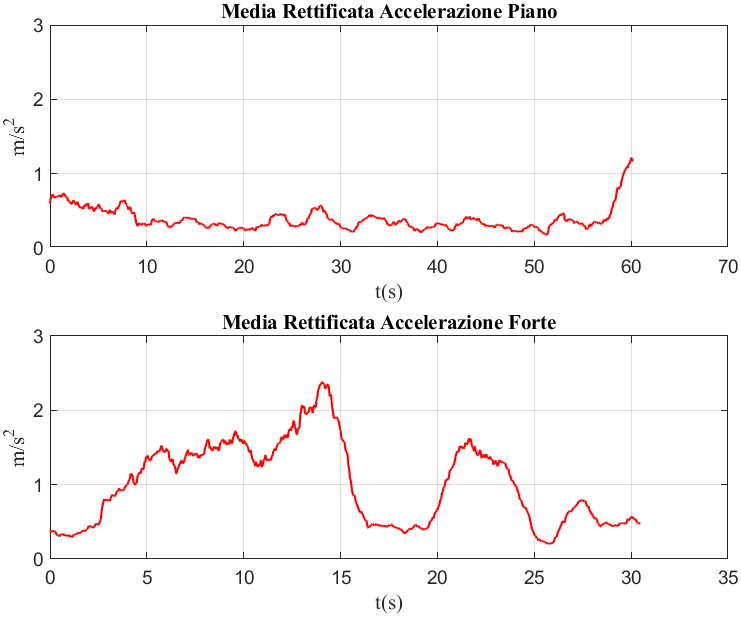
\includegraphics[height=.65\textheight]{figure/lungaFP_arvAccY}
		
		\vspace{.05\textheight}
		Questo indicatore è in grado di evidenziare le \textbf{accelerazioni evitando} di mostrare le \textbf{frenate}.
	\end{frame}
	
	\begin{frame}{{Varianza XY}}
		\centering\includegraphics[height=.65\textheight]{figure/lungaFP_varAccXY}
		
		\vspace{.05\textheight}
		Varianza degli ultimi 1.6s dell'accelerazione lungo X e Y.
		Dai grafici sì può notare come la \textbf{varianza in X} riesca a evidenziare sia le \textbf{accelerazioni} che le \textbf{frenate}, mentre quella in \textbf{Y} mostra solo le \textbf{accelerazioni}.
	\end{frame}
	
	\begin{frame}{{Deviazione Standard XY}}
		\vspace{.05\textheight}
		\centering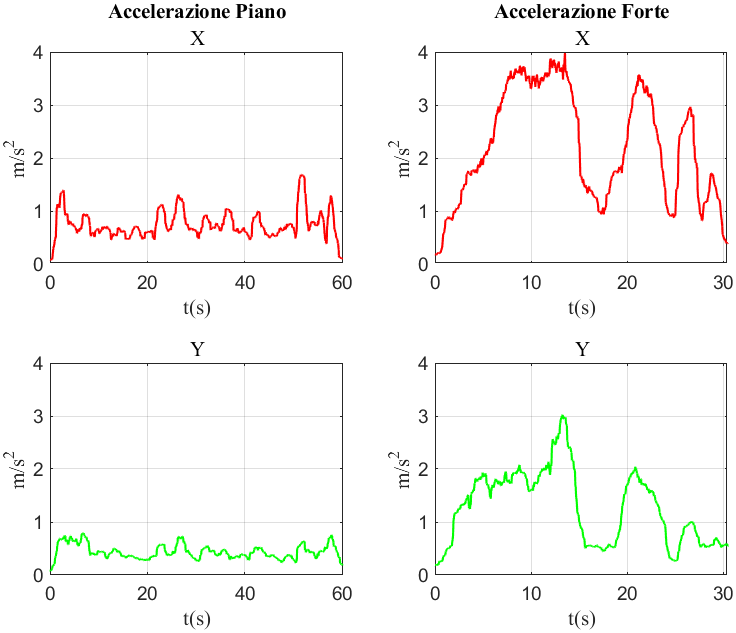
\includegraphics[height=.8\textheight]{figure/lungaFP_stdAccXY}
	\end{frame}
	
	\begin{frame}{{Scarto Quadratico Medio XY}}
		\vspace{.05\textheight}
		\centering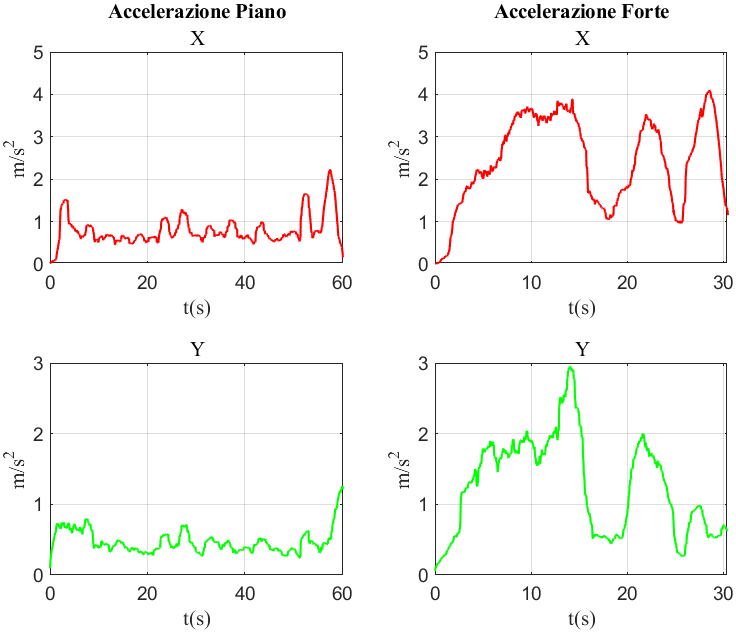
\includegraphics[height=.8\textheight]{figure/lungaFP_rmsAccXY}
	\end{frame}
	
	\begin{frame}{{Kurtosi XY}}
		\centering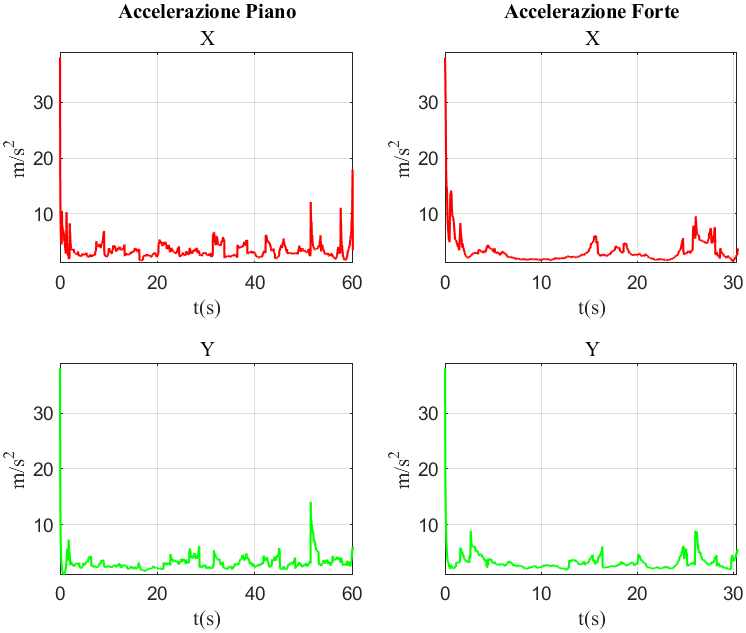
\includegraphics[height=.65\textheight]{figure/lungaFP_krtAccXY}	\vspace{.05\textheight}
		
		Per quanto riguarda percorsi dritti la kurtosi non sembra dare informazioni particolarmente interessanti.
	\end{frame}
	
	\begin{frame}{{Skewness XY}}
		\centering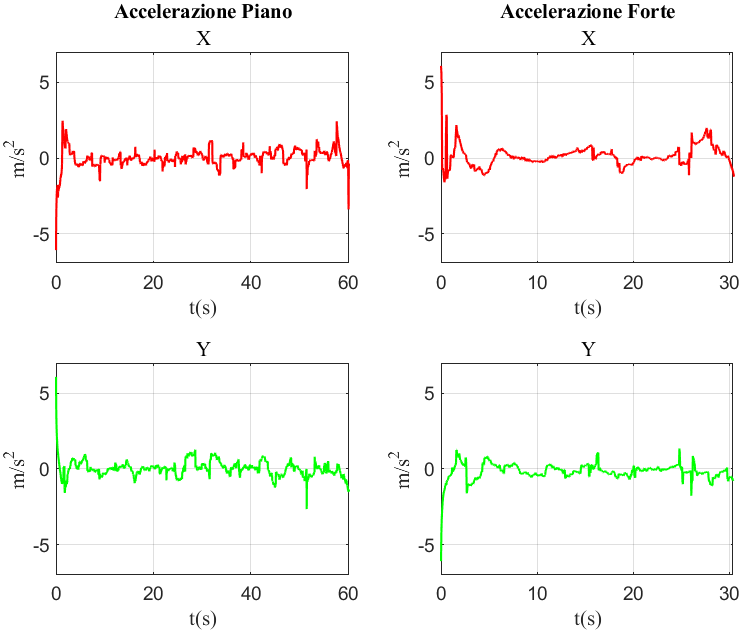
\includegraphics[height=.65\textheight]{figure/lungaFP_skwAccXY}	\vspace{.05\textheight}
		
		Come per la Kurtosi, anche la Skewness, percorsi dritti, non sembra dare informazioni particolarmente utili.
	\end{frame}
	
	\begin{frame}{{Max XY}}
		\centering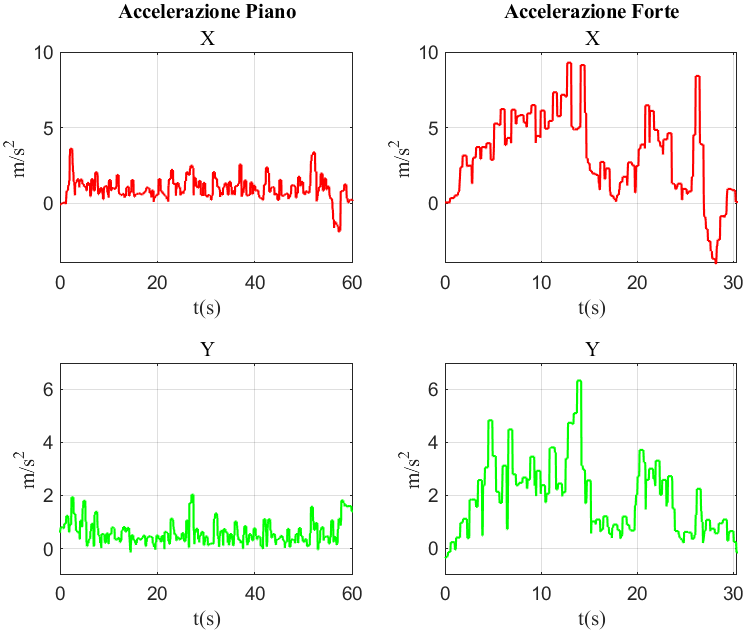
\includegraphics[height=.6\textheight]{figure/lungaFP_maxAccXY}	\vspace{.05\textheight}
		
		Il massimo degli ultimi 0.4s (10 dati).
		
		Il massimo di \textcolor{red}{\textbf{X}} è in grado di evidenziare sia le \textcolor{red}{\textbf{accelerazioni}} che le \textcolor{red}{\textbf{frenate}}. Queste ultime, al contrario di quanto avveniva per varianza, deviazione standard e scarto quadratico medio, vengono evidenziate con un valore \textbf{negativo}.
		
		Il massimo di \textcolor{green}{\textbf{Y}}, invece, evidenzia solo le \textcolor{green}{\textbf{accelerazioni}}.
		
	\end{frame}	
	
	\begin{frame}{{Min XY}}
		\centering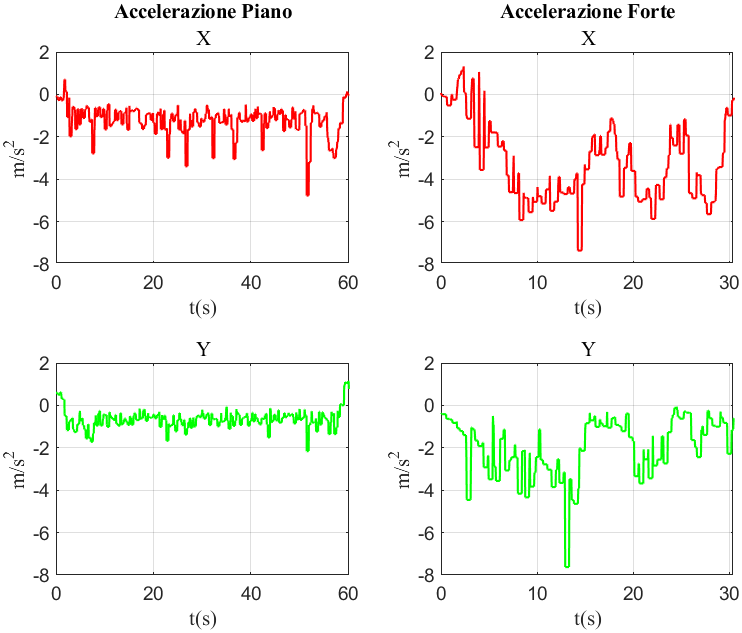
\includegraphics[height=.6\textheight]{figure/lungaFP_minAccXY}	\vspace{.05\textheight}
		
		Il minimo degli ultimi 0.4s (10 dati).
		
		Il minimo di \textcolor{red}{\textbf{X}} evidenzia sia le \textcolor{red}{\textbf{accelerazioni}} che le \textcolor{red}{\textbf{frenate}} come valori negativi, ma non è possibile distinguere tra le due.
		
		Il minimo di \textcolor{green}{\textbf{Y}}, invece, evidenzia solo le \textcolor{green}{\textbf{accelerazioni}}.
		
	\end{frame}
	
	\begin{frame}{{Distanza Picco-Picco XY}}
		\centering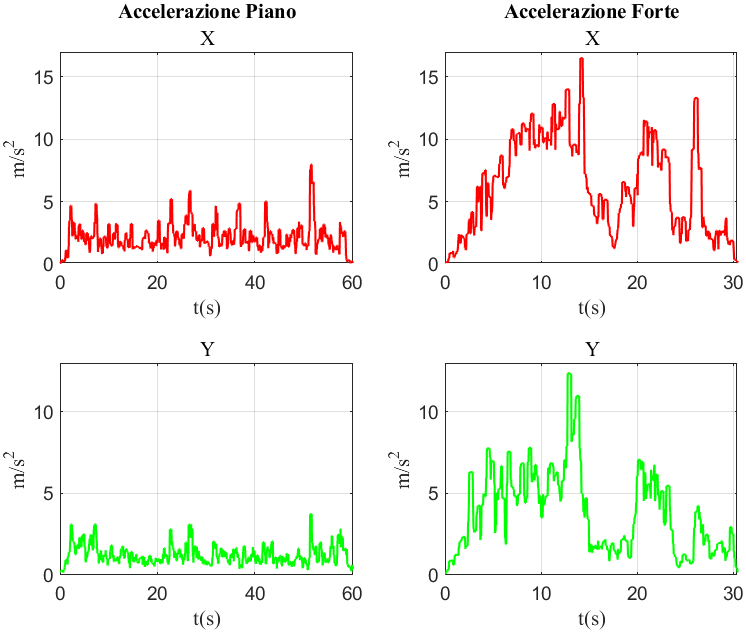
\includegraphics[height=.6\textheight]{figure/lungaFP_peak2peakAccXY}	\vspace{.05\textheight}
		
		La distanza picco-picco degli ultimi 0.4s (10 dati).
		
		La \textcolor{red}{\textbf{X}} è in grado di evidenziare \textcolor{red}{\textbf{accelerazioni}} e \textcolor{red}{\textbf{frenate}} ma, rispetto al massimo, perde la capacità di distinguere tra i due.
		
		La \textcolor{green}{\textbf{Y}}, invece, evidenzia solo le \textcolor{green}{\textbf{accelerazioni}}.
		
	\end{frame}	
	
	

	\begin{frame}{{Shape Factor XY}}
		\vspace{.05\textheight}
		\centering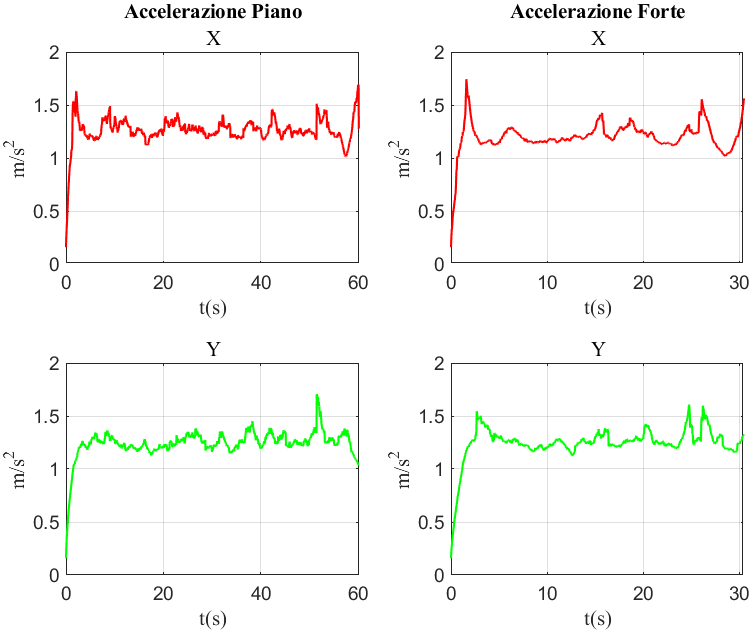
\includegraphics[height=.8\textheight]{figure/lungaFP_shfAccXY}	
	
	\end{frame}
	
	\begin{frame}{{Crest Factor XY}}
		\vspace{.05\textheight}
		\centering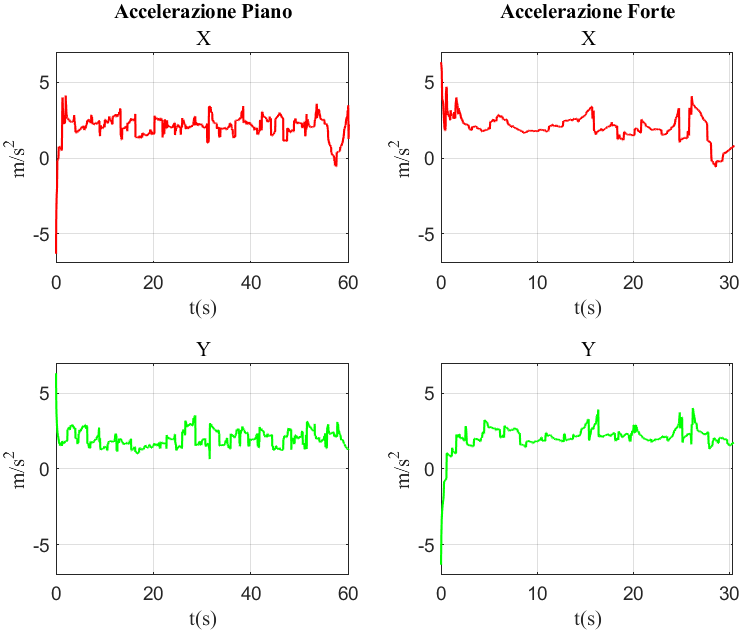
\includegraphics[height=.8\textheight]{figure/lungaFP_crfAccXY}	
		
	\end{frame}
	
	\begin{frame}{{Impulse Factor XY}}
		\vspace{.05\textheight}
		\centering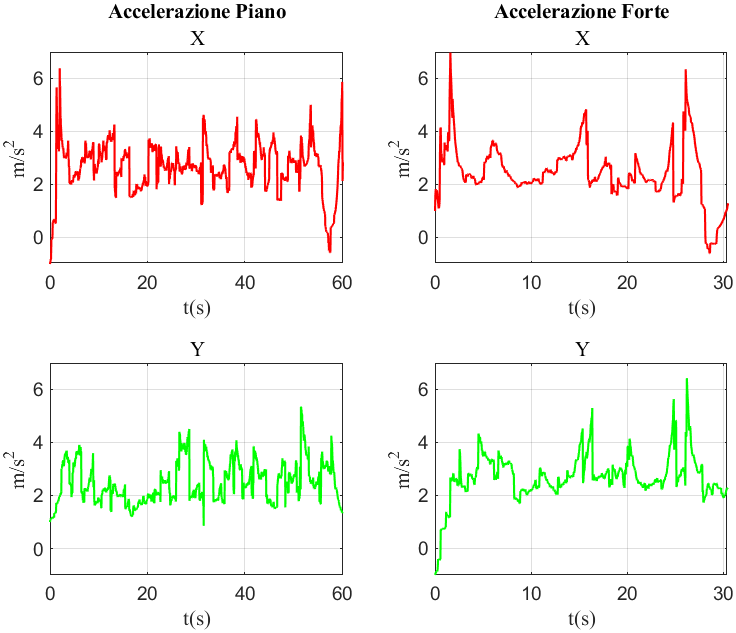
\includegraphics[height=.8\textheight]{figure/lungaFP_impfAccXY}	
		
	\end{frame}
	
	\begin{frame}{{Margin Factor XY}}
		\vspace{.05\textheight}
		\centering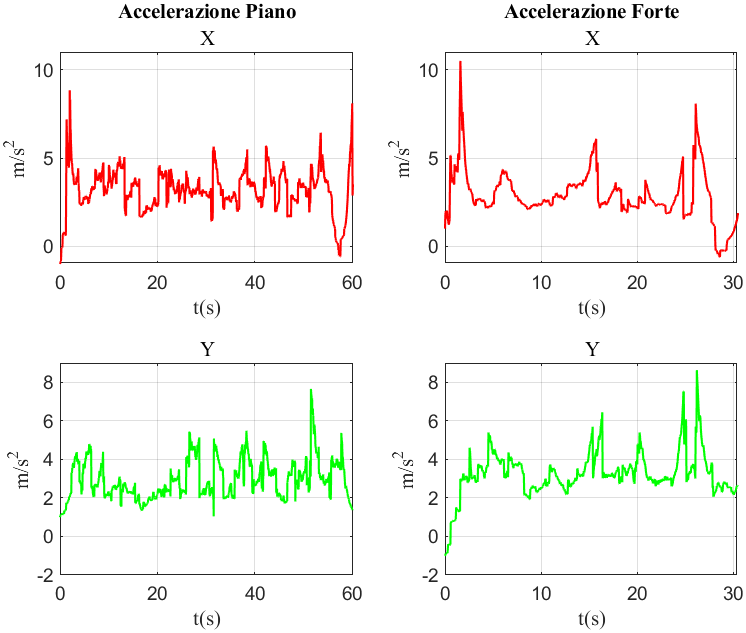
\includegraphics[height=.8\textheight]{figure/lungaFP_mrgfAccXY}	
		
	\end{frame}
	
	\begin{frame}{{Trasformata e Spettro Accelerazione X}}
		\centering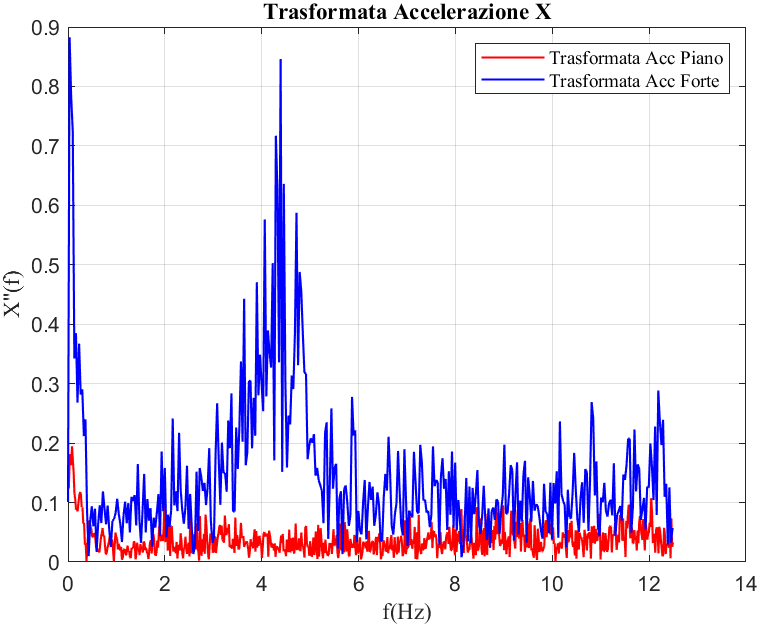
\includegraphics[width=.45\textwidth]{figure/lungaFP_TrasfAccX}
		\hspace{.05\textwidth}
		\centering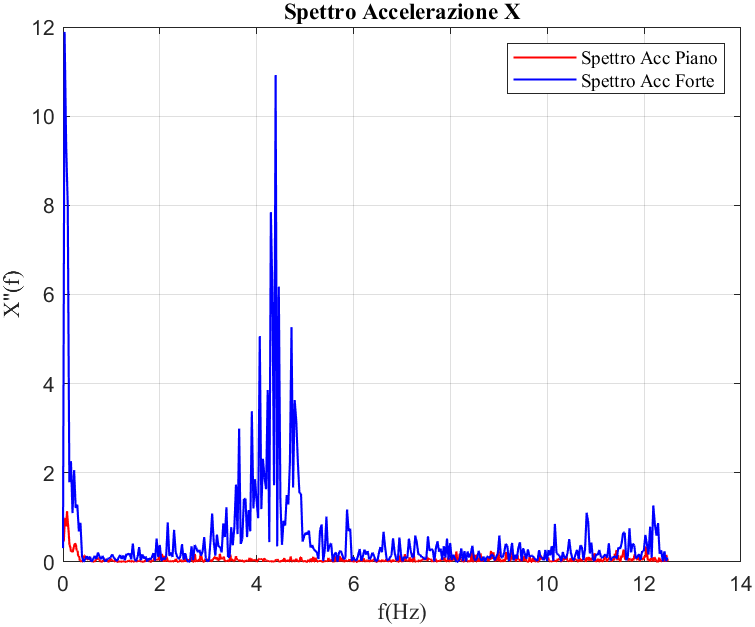
\includegraphics[width=.45\textwidth]{figure/lungaFP_SpettroAccX}
		\vspace{.05\textheight}
		
		A \textbf{sinistra} la \textbf{trasformata} dell'accelerazione in \textbf{X}, a \textbf{destra} lo \textbf{spettro}.
		Come si può notare dai grafici durante una pedalata \textcolor{blue}{forte} si ha un \textcolor{blue}{incremento delle frequenze tra i 2 e i 6Hz}. In caso di pedalate leggere le frequenze interessate si abbassano.
	\end{frame}
	
	\begin{frame}{{Trasformata e Spettro Accelerazione Y}}
		\centering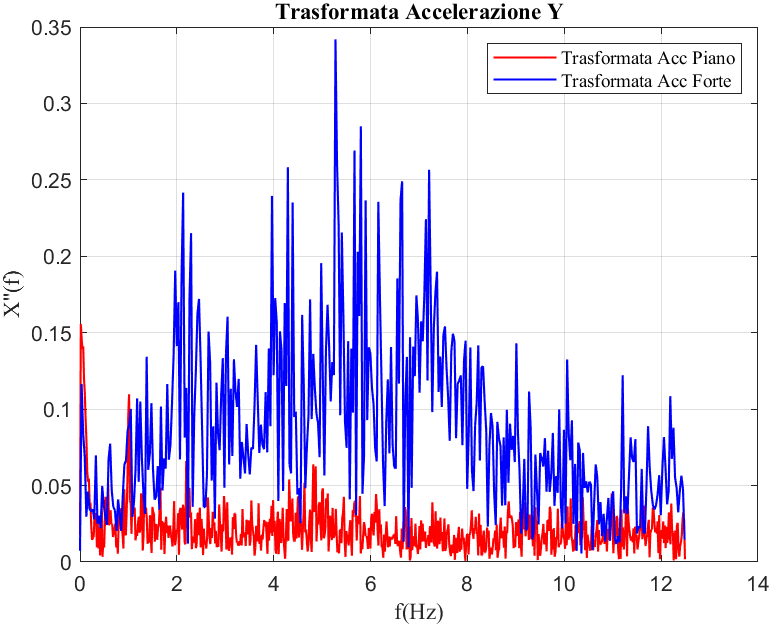
\includegraphics[width=.45\textwidth]{figure/lungaFP_TrasfAccY}
		\hspace{.05\textwidth}
		\centering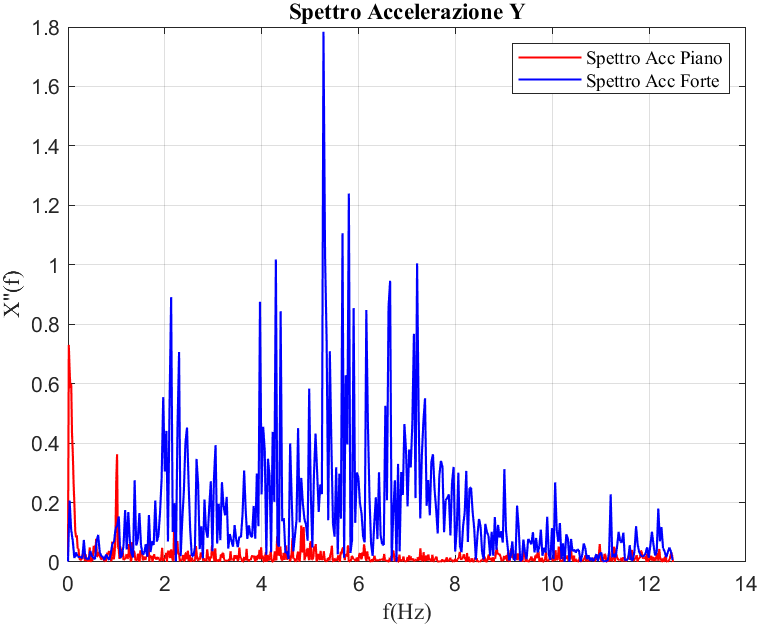
\includegraphics[width=.45\textwidth]{figure/lungaFP_SpettroAccY}
		\vspace{.05\textheight}
		
		A \textbf{sinistra} la \textbf{trasformata} dell'accelerazione in \textbf{Y}, a \textbf{destra} lo \textbf{spettro}.
		Come si può notare dai grafici durante una pedalata \textcolor{blue}{forte} si ha un \textcolor{blue}{incremento generale delle frequenze}, che va a diminuire nel caso di pedalate leggere.
	\end{frame}
	
	\begin{frame}{{Accelerazione X Filtrata}}
		\centering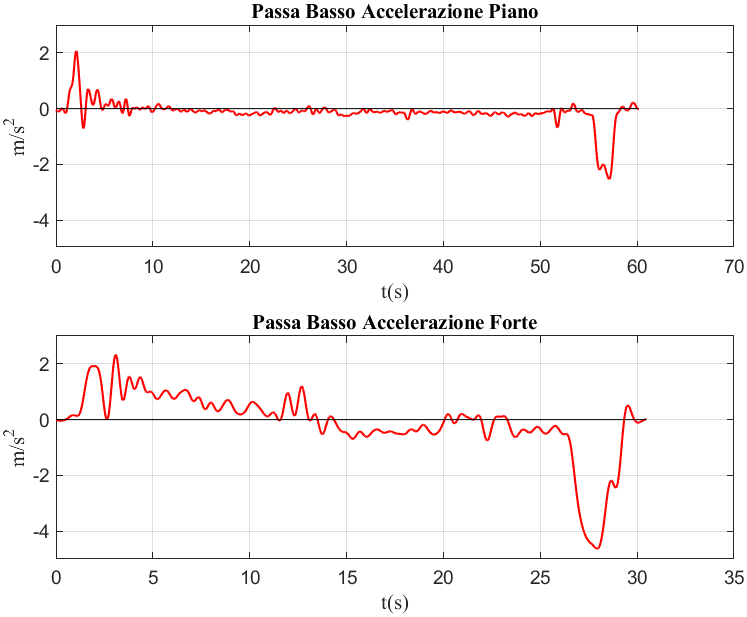
\includegraphics[height=.65\textheight]{figure/lungaFP_LowPassAccX}	\vspace{.05\textheight}
		
		Accelerazione \textbf{X filtrata a 0.5Hz} tramite \textbf{filtro passa-basso} per \textbf{rimuovere dalle misure} i \textbf{"disturbi" dovuti alle pedalate}.
	\end{frame}
	
	\begin{frame}{{Accelerazione Y Filtrata}}
		\centering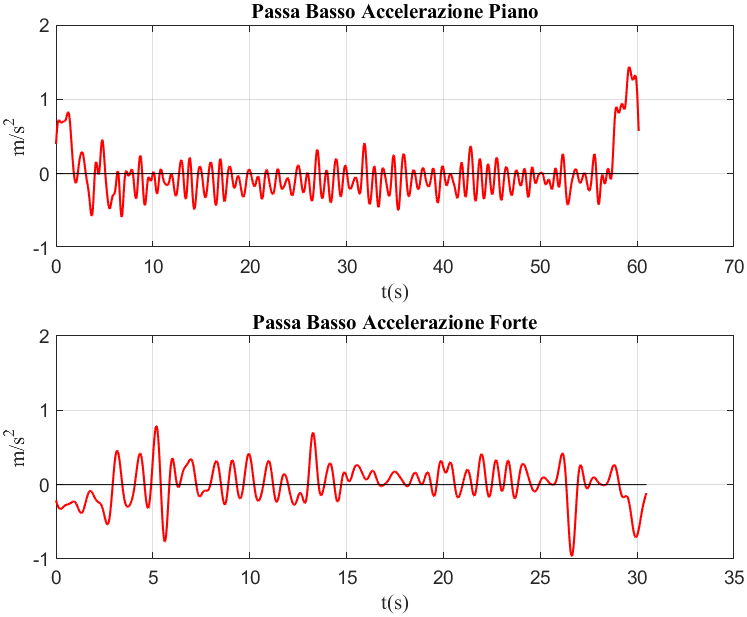
\includegraphics[height=.65\textheight]{figure/lungaFP_LowPassAccY}	\vspace{.05\textheight}
		
		Accelerazione \textbf{Y filtrata a 0.5Hz} tramite \textbf{filtro passa-basso} per \textbf{rimuovere dalle misure} i \textbf{"disturbi" dovuti alle pedalate}.
	\end{frame}
	
	\begin{frame}{{Mancanti}}
		\centering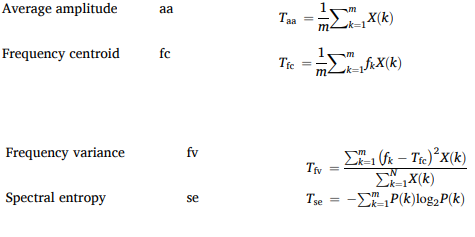
\includegraphics[width=.80\textwidth]{figure/mancanti}
		\vspace{.05\textheight}
		
		Grafici che devono ancora essere inseriti.
		
		
	\end{frame}
	
	
\end{document}